\documentclass[16pt,a4paper]{article}

\usepackage{fontspec}
\setmainfont[BoldFont=黑体]{方正新书宋简体}          
\XeTeXlinebreaklocale "zh"                    
\XeTeXlinebreakskip = 0pt plus 1pt minus 0.1pt  

\usepackage{indentfirst} 
\setlength{\parindent}{2em}

\usepackage{changepage}
\usepackage{float}
\usepackage{setspace}
\usepackage{amsmath}
\usepackage{amsfonts}
\usepackage{amssymb}

\usepackage{geometry}
\geometry{left=2.5cm,right=2.5cm,top=2.5cm,bottom=4cm}
\usepackage{fancyhdr}
\pagestyle{fancy}
\lhead{\includegraphics[scale=0.5]{logo.png}}

\author{郭嘉丞 \quad 姚皓天}
\title{数字听诊器 \\ Digital Stethoscope}
\date{2015年6月}

\graphicspath{{Figure/}}

\begin{document}
\maketitle
\thispagestyle{empty}
\newpage
\section{简介}

\section{系统设计}


\section{硬件设计细节}
\subsection{电源部分}
电源是系统中容易被忽视,但是又非常重要关乎系统性能的关键部分。\\
本设计中含有数字部分和模拟部分,各自使用独立的电源:
\begin{itemize}
\item 数字部分采用 Step-Down(Buck) Converter
\item 模拟部分采用 High PSRR, Low Noise, Single Output LDO
\end{itemize}

\subsubsection{数字电源}
\begin{figure}[H]
\centering
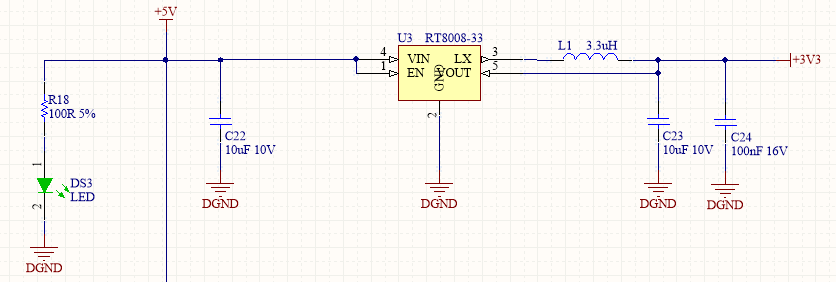
\includegraphics[width=0.8\textwidth]{power1.png}
\caption{开关电源} 
\end{figure}
数字部分采用Richtek RT8008-3.3供电。这款芯片具有以下特点:
\begin{enumerate}
\item 固定输出电压3.3V
\item 1.5MHz的PWM频率,可以使用小型的外部电感和电容
\item 内置场效应管,采用同步整流方式,具有较高的效率
\end{enumerate}\par
由于具有效率高,体积小,占用PCB面积小的特点,非常适合为本设计的数字部分供电,也利于手持设备小型化。\par
图中DS3用作电源指示灯。

\subsubsection{模拟电源}
\begin{figure}[H]
\centering
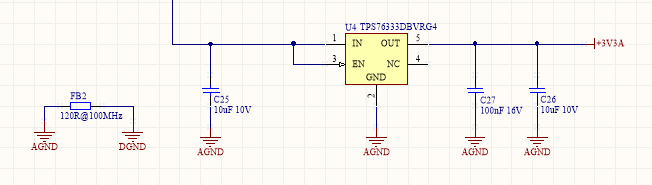
\includegraphics[width=0.8\textwidth]{power2.png}
\caption{线性电源} 
\end{figure}
模拟部分采用TI TPS79333供电。这款芯片具有以下特点:

\begin{enumerate}
\item 高PSRR(70 dB at 10 kHz)
\item 低噪声(32 $\mu V_{RMS}$)
\end{enumerate}\par
该芯片可以有效抑制电源噪声,提供符合模拟部分工作的低噪声电源。\par
图中FB2 采用120R@100MHz的磁珠将模拟地与数字地相连,可以避免数字部分对模拟部分的干扰。
\subsection{模拟前端和数据转换}


\subsection{微控制器}
\subsection{其他数字外设}


\end{document}
